\section{Design}
\label{sec:design}
The design of the \gls{its} shown in Figure~\ref{fig:its-overview} extends the existing functionality of the training platform.
This existing functionality is depicted in orange on the right side of the figure, while components of the \gls{its} are drawn in blue on the left side.
The \gls{its} consists of two loops, it contains three algorithmic components and three types of data collections.

% high level overview of different components of ITS
\begin{figure}
    \centering
    %\input{03-education/plots/its-flowchart-reverse}
    \includegraphics[page=12]{03-education/figures/tikzfigures.pdf}
  \caption[Design of the ITS]{The \Gls{its} consists of two loops. In the main loop, users are served exercises and their answers are processed, before selecting a new exercise. The user history is then regularly used in a secondary loop to estimate both user abilities and exercise difficulties.}
  \label{fig:its-overview} 
\end{figure}

The algorithmic component in the main loop is that of exercise selection.
Selecting the optimal exercise is done through an adapted \gls{cf} algorithm, as will be explained in more detail in Section~\ref{sec:collab}.
In this technique, a recommendation is derived from historical data of like-minded users.
To evaluate this technique, and hence improve it, we need a measure to decide what a good recommendation is.

A useful challenge is a challenge from which the user has learned something and that keeps the user engaged.
That is, a good recommendation system should increase the \textit{ability} of the user, and their \textit{engagement}.
It is easy to keep track of the engagement of the user.
If they continue to play more challenges, that means they stay engaged.
However, in order to determine if a recommendation leads to increased ability, we need to be able to continuously measure the ability of each user.
Another reason to continuously measure the ability of each user is the temporal aspect to learning.
An exercise that is useful to a user at the beginning of their journey is likely no longer an appropriate recommendation once their ability has sufficiently increased.
Hence ability estimation is needed to both determine \textit{if} a challenge was useful to a user, and \textit{when} a challenge was useful.

A very naive way to achieve an ability estimate is simply looking at the accuracy of each user.
A user answering all of the challenges correctly (100\% accuracy), is likely to have a higher ability level than a user answering half of them correctly (50\% accuracy).
If all users completed the exact same challenges, this could give a reasonably accurate representation of their ability level.
In fact, that is exactly the reasoning behind \gls{ctt}~\cite{ctt}.
In a classic test all examinees are given the same (or equivalent) exercises and their accuracy on the test is an indication of their ability level.

However, on the training platform not all users are completing the exact same challenges and this is not desirable, as that would conflict with the goal of individually tailored recommendations.
When users are completing different challenges, accuracy alone is no longer sufficient.
It is possible for one user to maintain a high accuracy doing simple challenges, while another user's accuracy is lower but they are completing difficult challenges.

This is also true for exercises, the difficulty of an exercise can not be accurately estimated through the accuracy of users completing it.
It is possible for one exercise to have a high accuracy because it is mostly attempted by users of a high ability level, while another is often tried by beginners and hence has a lower accuracy.
It is clear that these two remaining algorithmic components in the \gls{its} are tightly coupled.
Both are implemented through the use of psychometric models from the field of \gls{irt} as explained in Section~\ref{sec:calib}.
The calibration techniques of \gls{irt} use the entire user history and take a while to complete.
This is why they are not performed every iteration of the main loop, but at regular intervals in a secondary loop.
